\chapter{Implementation}\label{chapter:implementation}

Focaccia is a Python application. This section details some notable points of its implementation.

\section{Tools}

\subsection{Symbolic Execution Backend}

A symbolic execution backend, in order to be useful for our specific purpose, must satisfy multiple conditions:

\begin{itemize}
    \item Symbolic execution for assembly languages (many tools operate on high-level languages); primarily x86, but
        preferredly more
    \item Python API
    \item Freedom to execute single instructions symbolically on arbitrary states
    \item Low-level access to generated symbolic expressions
\end{itemize}

The first tool in consideration was the binary analysis framework \textit{angr}~\cite{shoshitaishvili2016state}. angr is
a mature and well-tested open source platform for control-flow graph recovery, symbolic execution, disassembly and
lifting, and more~\cite{AngrWebsite2024Mar}. Still, angr ended up being rejected for the use as Focaccia's symbolic
execution backend. Almost none of our tasks were easily accomplished with angr; the interface is so tuned to high-level
cyber security tasks that our attempts to accomplish `just this one simple thing' grew into a constant battle against
the API\@. Not only does angr bury its low-level functionality, which would have sufficed for Focaccia's purposes, under
huge stacks of abstraction, delegation, and opaqueness, but also turned out to be slow while doing that.

Further research has led us to adopt Miasm~\cite{desclaux2012miasm}, a reverse engineering framework developed by CEA IT
Security at the French Alternative Energies and Atomic Energy Commission. Its features include
opening/modifying/generating binary files, assembling/disassembling a host of assembly languages, emulation, symbolic
execution, and \textbf{representing assembly semantics using an intermediate language}~\cite{cea-sec2024Mar}. The latter
statement hints towards exactly the functionality that Focaccia requires.

As a proposal for future improvement of Focaccia, it is entirely possible to build a custom abstraction layer over the
symbolic execution backend as a means to have multiple interchangeable backends for feature- and implementation
completeness of all desired architectures. We discarded this idea initially for its likelihood to incur unnecessary
effort, though the evaluation has shown that the backend's completeness really is a major pain point of Focaccia.

\subsection{Concrete Execution Tracer}

We need to follow a program's native execution on a per-instruction basis and inspect the program's state at each trace
point (see section~\ref{sec:concolic_tracing}). A debugger is a canonical choice for this task; we use LLDB because it
has a Python API (one can start and manipulate debugger instances conveniently in Python code)~\cite{lldb2024Apr}.

\section{Algorithms}\label{sec:algorithms}

\subsection{Generating Symbolic Expressions}\label{sec:symb_expr_impl}

The goal for transforming instructions to symbolic expressions is to generate equations that are, despite being guided
to a certain extent by the native execution's concrete reference state, as symbolic as possible. Ideally, the concrete
state's only purpose would be to indicate for which instructions symbolic expressions are to be generated, which is
indeed possible for the most part. For example, an \texttt{ADD} instruction always performs the same conceptual
operation for each configuration of operand types (memory, register, or immediate), no matter the concrete values of the
program state on which it is executed. Conditional instructions like \texttt{CMOVcc}, on the other hand, modify their
behaviour based on the condition operand's concrete value. The first iteration of the implementation inspected the
concrete state to resolve to which location the instruction writes: \texttt{CMOVNZ RDX, RAX} would generate the equation
\texttt{RDX = RAX} if \texttt{ZF = 0} in the concrete reference state, and \texttt{RDX = RDX}
otherwise~\cite{Intel2023DeveloperManualVol1}.  However, the formula can be improved to be less reliant on concrete
state, thereby increasing the number of test cases it can verify correctly, if our symbolic language has support for
conditional expressions. This is the case with Miasm. An improved version of the algorithm generates for the same
instruction the equation \texttt{RBX = (ZF == 0) ? RAX : RBX}. No concrete state is considered at all---the equation is
perfectly symbolic and captures all possible scenarios.

The perfectly abstract approach does not work for all instructions: Repeated string instructions like \texttt{REP STOS},
where the number of loop iterations depends on the initial state, can not be captured in a finite formula because they
do not necessarily terminate for all inputs---at least not in a realistic amount of time and with realistic space
consumption: an equation for a possible loop count of $2^{64} - 1$ on 64-bit architectures is theoretically but not
practically representable or even computable. For these instructions, the concrete reference execution is used as a
termination condition: the generated equation will always have a number of iterations matching the expected number for
its specific initial state. This is a severe limitation on its verification power, though not circumventable.
\lstlistingname~\ref{fig:symb_equation_loop} shows an example.

\begin{figure}[htbp]
    \centering
    \begin{tabular}{c}
    \texttt{REP STOS es:[RDI] EAX} \\
    \midrule
    \begin{lstlisting}
        RDI        = RDI + 0x130
        RCX        = RCX + 0xFFFFFFFFFFFFFFB4
        @32[RDI]   = RCX ? (RAX[0:32], @32[RDI])
        @32[RDI + 0x4]  = (RCX == 0x1) ? (@32[RDI + 0x4],  RAX[0:32])
        @32[RDI + 0x8]  = (RCX == 0x2) ? (@32[RDI + 0x8],  RAX[0:32])
        @32[RDI + 0xC]  = (RCX == 0x3) ? (@32[RDI + 0xC],  RAX[0:32])
        @32[RDI + 0x10] = (RCX == 0x4) ? (@32[RDI + 0x10], RAX[0:32])
        ...
    \end{lstlisting}
    \end{tabular}
    \caption[]{Symbolic equations for \texttt{REP} instruction}\label{fig:symb_equation_loop}
\end{figure}

The Miasm backend lifts parsed instructions to an \ac{IR} on which the symbolic execution engine operates. For
semantically complex instructions like the latter two described above, it generates multiple \ac{IR} blocks that are
chained together, forming an \ac{IR} control flow graph; Figures~\ref{fig:ir_graph_cmov} and~\ref{fig:ir_graph_repstod}
show examples of these IR graphs for instructions \texttt{CMOVNZ RDX, RAX} and \texttt{REP STOS es:[RDI], EAX},
respectively.

For our purposes, we want to collapse the entire graph into a unified collection of assignment statements, such that
\figurename~\ref{fig:ir_graph_repstod} produces the symbolic equations shown in
\figurename~\ref{fig:symb_equation_loop}. We accomplish this with a small symbolic interpreter that traverses the graph
(i.e., executes the graph purely symbolically) and collects the visited nodes' modifications to the program state. If a
branch is encountered, instead of deciding on a path to take, both destinations are considered and combined into a
single conditional assignment, thus avoiding the need to consider concrete state to decide the branch condition. As
noted before, this works because a single instruction's internal branching behaviour is usually simple enough not to
induce explosive path growth. \figurename~\ref{fig:symb_branch_to_assign} shows this transformation for the
\texttt{CMOVNZ RDX, RAX} example. The left side shows the instruction's semantics as pseudocode, the right side shows
the resulting conditional assignment. As a reference, \figurename~\ref{fig:ir_graph_cmov} visualizes the instruction's
IR graph as generated by the Miasm backend.

\begin{figure}[htpb]
    \begin{subfigure}[b]{0.3\linewidth}
        \begin{lstlisting}
            if not ZF:
                RDX = RAX
        \end{lstlisting}
        \caption{Branch}\label{fig:symb_conditional_1}
    \end{subfigure}
    \hfill
    \begin{subfigure}[b]{0.5\linewidth}
        \begin{lstlisting}
            RDX = ZF ? RDX : RAX
        \end{lstlisting}
        \caption{Combined Conditional Assignment}\label{fig:symb_conditional_2}
    \end{subfigure}
    \caption{Transforming Branches to Conditional Assignments}\label{fig:symb_branch_to_assign}
\end{figure}

\begin{figure}[htpb]
    \centering
    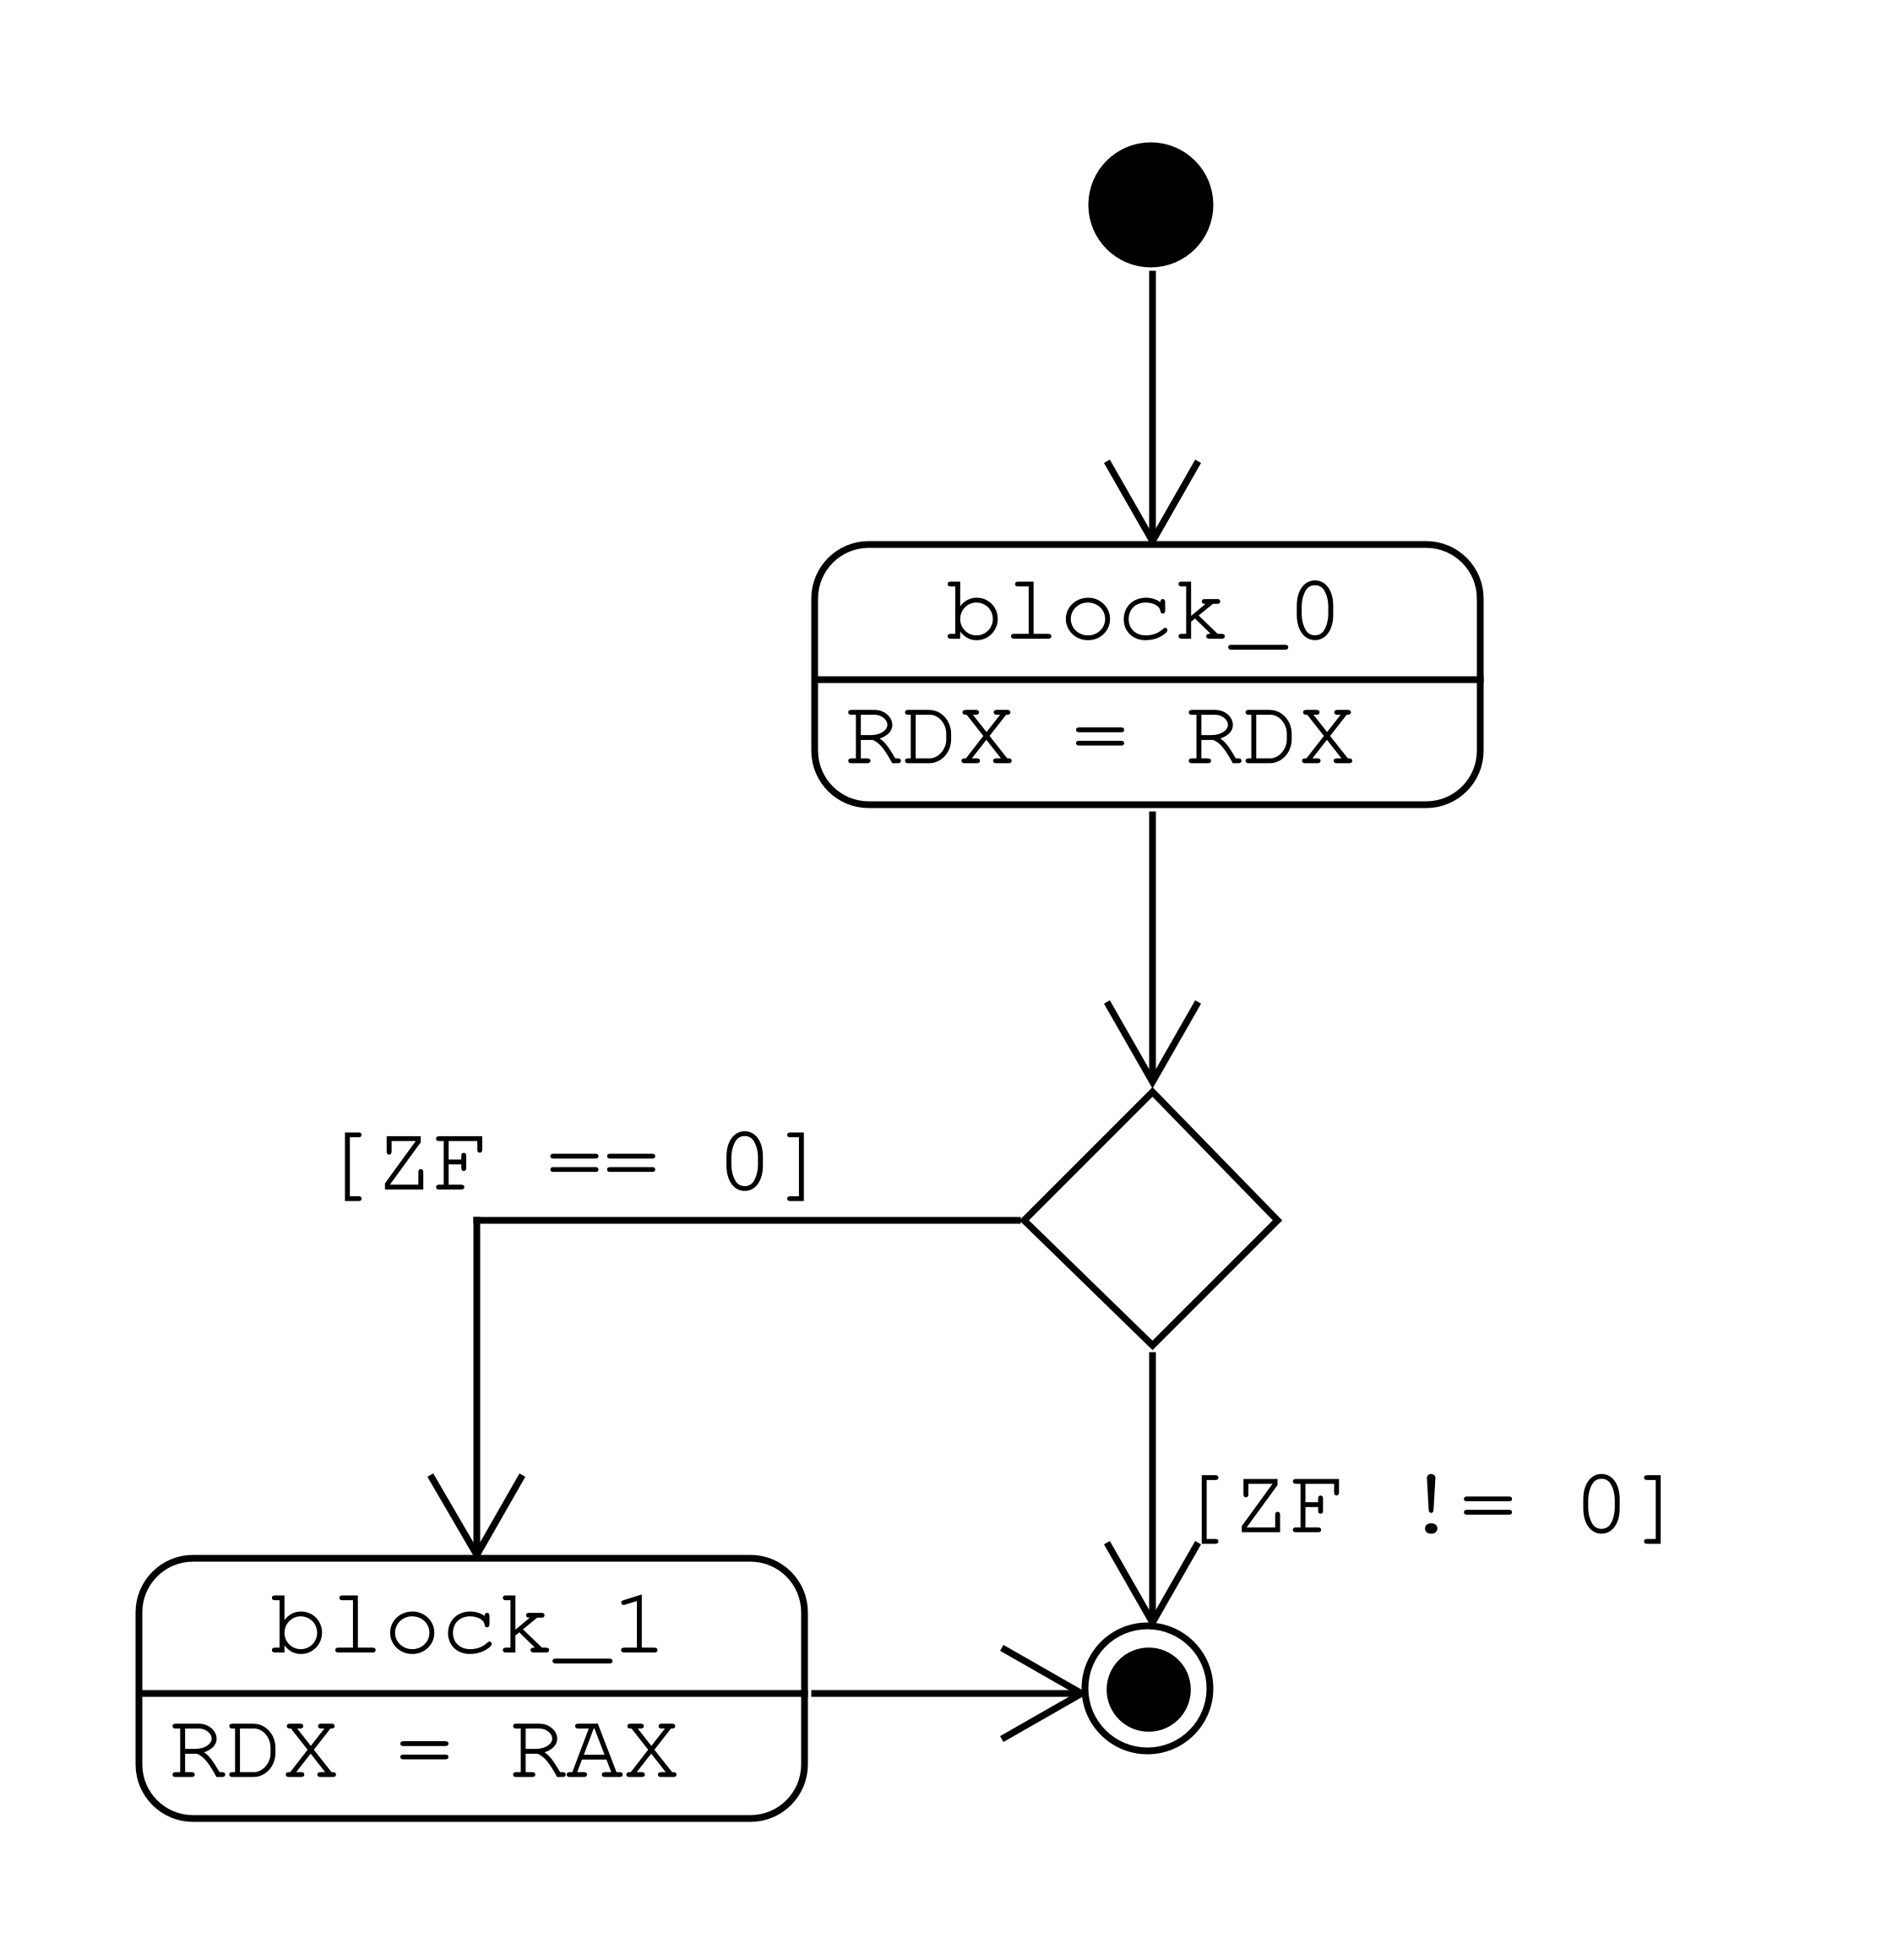
\includegraphics[width=0.5\linewidth]{figures/ir_graph_cmov.png}
    \caption{IR graph for \texttt{CMOVNZ RDX, RAX}}\label{fig:ir_graph_cmov}
\end{figure}

\begin{figure}[htpb]
    \centering
    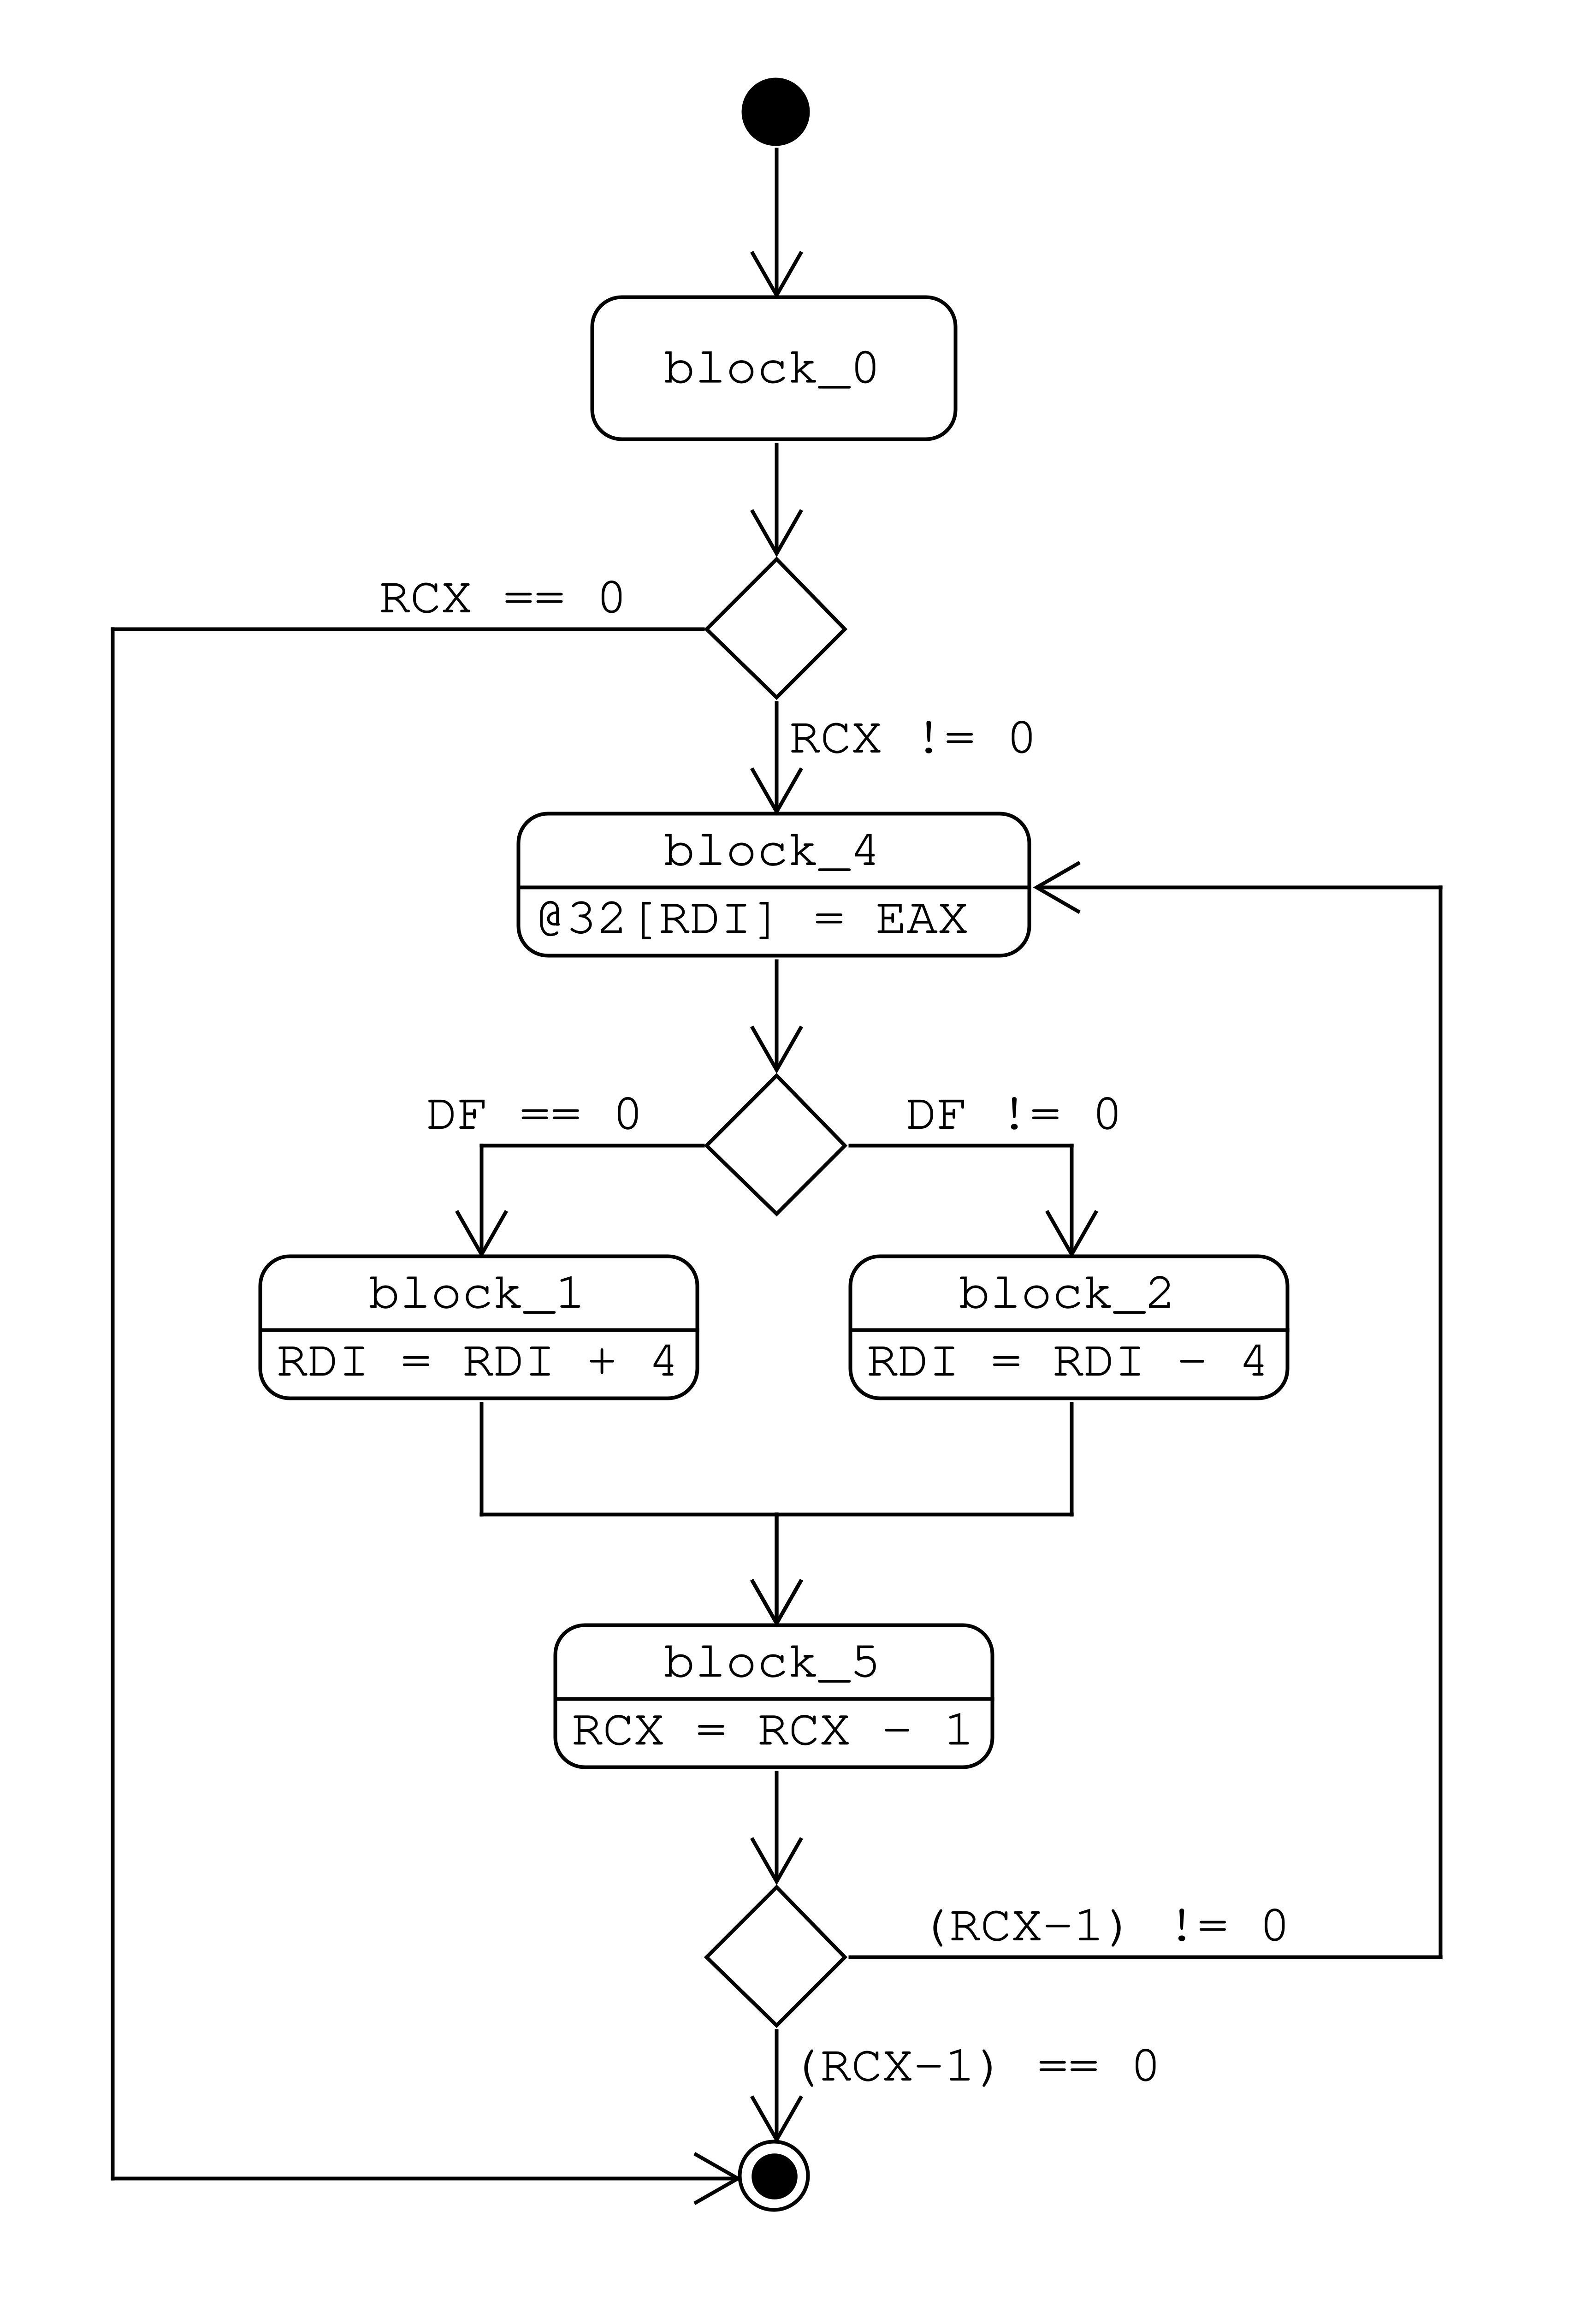
\includegraphics[width=0.7\linewidth]{figures/ir_graph_repstosd.png}
    \caption{IR graph for \texttt{REP STOSD}}\label{fig:ir_graph_repstod}
\end{figure}

To handle the complex case of loops, the branch destinations of branches that are encountered repeatedly are concretized
to a single IR block by taking into account the concrete guidance state. This decides possibly unhalting loop
termination conditions and is the only case where concrete state is considered during symbolic expression generation.

\subsection{Calculating Truth States}

The process of computing truth states by applying symbolic expressions to initial states is comparatively
straightforward. For any symbolic assignment statement (symbolic representations of instructions consist only of
assignments at the top level, either to registers or to memory locations), a small interpreter walks through the right
hand side's syntax tree and replaces all symbolic references to registers or memory locations (the addresses of which
are resolved to concrete values the same way) with concrete values from the initial program state to which the symbolic
expression is applied. Once the expression is devoid of symbols, an expression simplifier provided by the backend can
collapse complex arithmetic expressions or bitvector-accesses to single values. The assignment destination in the
updated state, determined by the assignment's left hand side to which the same process is applied in case it is a
complex expression, is updated with this value.

\subsection{Verifying a Program State's Correctness}

The comparison of states is similarly uncomplicated. For any pair of emulator states $(S^E_i, S^E_{i+1})$ and a symbolic
transformation $\sigma_i : S^E_i \mapsto S'_{i+1}$ we use that transformation to calculate the expected state
$S'_{i+1}$, then test whether all values that were \textit{modified} by $\sigma_i$ are equal to the respective values in
the emulator state $S^E_{i+1}$.

Errors of different severity levels are generated depending on the type of error found: A common warning that is not a
definite error in the emulator is insufficient data (that is, any of the emulator states don't contain data required by
the transformation or the comparison), which may happen if the emulator's log is incomplete or other complications occur
in the communication of the emulator's states.

\section{Details}\label{sec:impl_details}

\subsection{Environmental Differences: The Auxiliary Vector}\label{sec:auxv}

A curious source of difference in branching behaviour (as discussed in section~\ref{sec:trace_mismatch}) between
concrete- and emulator execution is the auxiliary vector on Linux systems, which is "a mechanism that the kernel's ELF
binary loader uses to pass certain information to user space when a program is executed"~\cite{getauxval2024Mar}. Libc's
initialization code (at least glibc as well as musl libc~\cite{MuslLibc2024Feb}) iterates over that array to bring it
into a representation that is indexable by entry names, thereby depending its branching behaviour on the array's size.
It turns out that QEMU, at least on some systems, passes an auxiliary vector to the application that is different from
the native auxiliary vector on the same system; \figurename~\ref{fig:auxv_comparison} shows an example. While a
customized launcher that starts both the tested emulator and the symbolic trace recorder could in theory ensure equal
environment arrays, the same is not possible for the kernel-provided auxiliary vector.

This shows that branch-based trace mismatches are not a rare phenomenon.

\begin{figure}[htpb]
    \begin{subfigure}[t]{0.4\linewidth}
        \begin{lstlisting}
            AT_BASE : 0x790a3a4f3000
            AT_CLKTCK : 0x7ffd4e2f21b9
            AT_EGID : 0x3e8
            AT_ENTRY : 0x5d141499c050
            AT_EUID : 0x3e8
            AT_EXECFN : 0x7ffd4e2f2fec
            AT_FLAGS : 0x0
            AT_GID : 0x3e8
            AT_HWCAP : 0x64
            AT_HWCAP2 : 0x2
            AT_MINSIGSTKSZ : 0x7f0
            AT_PAGESZ : 0x1000
            AT_PHDR : 0x5d141499b040
            AT_PHENT : 0x38
            AT_PHNUM : 0xd
            AT_PLATFORM : 0xbfebfbff
            AT_RANDOM : 0x7ffd4e2f21a9
            AT_RSEQ_ALIGN : 0x20
            AT_RSEQ_FEATURE_SIZE : 0x1c
            AT_SECURE : 0x0
            AT_SYSINFO_EHDR : 0x7ffd4e349000
            AT_UID : 0x3e8
        \end{lstlisting}
    \caption{Native AUXV}
    \label{fig:native_auxv}
    \end{subfigure}
    \hfill
    \begin{subfigure}[t]{0.4\linewidth}
        \begin{lstlisting}
            AT_BASE : 0x2aaaab2ac000
            AT_CLKTCK : 0x2aaaab2ab7f9
            AT_EGID : 0x3e8
            AT_ENTRY : 0x555555557050
            AT_EUID : 0x3e8
            AT_EXECFN : 0x2aaaab2abfd1
            AT_FLAGS : 0x0
            AT_GID : 0x3e8
            AT_HWCAP : 0x64
            AT_PAGESZ : 0x1000
            AT_PHDR : 0x555555556040
            AT_PHENT : 0x38
            AT_PHNUM : 0xd
            AT_PLATFORM : 0xfcbfbfd
            AT_RANDOM : 0x2aaaab2ab7e0
            AT_SECURE : 0x0
            AT_SYSINFO_EHDR : 0x2aaaab2e3000
            AT_UID : 0x3e8
        \end{lstlisting}
        \caption{QEMU's AUXV}
        \label{fig:qemu_auxv}
    \end{subfigure}
    \caption{Comparison of auxiliary vectors in native execution and QEMU}
    \label{fig:auxv_comparison}
\end{figure}
